\documentclass[12pt]{article}

% Computational Physics by M. Newman
% Setup file for exercises

% Packages
\usepackage{mathpazo}
\usepackage{amsmath}
\usepackage{graphicx}
\usepackage{calrsfs}
\usepackage{fancyvrb}

% Formatting
\setlength{\textwidth}{17.5cm}
\setlength{\textheight}{24.0cm}
\setlength{\evensidemargin}{2.5cm}
\setlength{\oddsidemargin}{-0.6cm}
\setlength{\topmargin}{-2.3cm}
\setlength{\textfloatsep}{0pt}
\setcounter{secnumdepth}{0}
\renewcommand{\baselinestretch}{1.06}

% Macros
\newcommand{\dd}{\mathrm{d}}
\newcommand{\ii}{\mathrm{i}}
\newcommand{\e}{\mathrm{e}}
\newcommand{\half}{\tfrac12}
\newcommand{\av}[1]{\langle#1\rangle}
\newcommand{\var}{\mathop\mathrm{var}}
\newcommand{\Ord}{\mathrm{O}}
\renewcommand{\Re}{\mathop\mathrm{Re}\nolimits}
\renewcommand{\Im}{\mathop\mathrm{Im}\nolimits}
\newcommand{\mat}{\mathbf}
\renewcommand{\vec}{\mathbf}
\newcommand{\defn}{\textit}
\newcommand{\exskip}{\nopagebreak\medskip\noindent}
\newcommand{\pmstrut}{\rule{0pt}{13pt}}

% Environments
\newcounter{chapter}
\setcounter{chapter}{2}
\newcounter{exercise}
\renewcommand{\theexercise}{\arabic{chapter}.\arabic{exercise}}
\newenvironment{exercises}{\vspace{2ex plus0.5ex minus0.5ex}
  \renewcommand{\labelenumi}{\alph{enumi})}}%
    {\par\vspace{1ex plus0.5ex minus0.5ex}}
\newcommand{\exercise}{\refstepcounter{exercise}%
  \par\vspace{4ex plus1ex minus1ex}%
  \noindent\textbf{Exercise \theexercise: }}

\DefineVerbatimEnvironment{code}{Verbatim}{xleftmargin=\parindent}

\setcounter{chapter}{4}

\begin{document}

\noindent {\LARGE\textsc{Computational Physics}}\par
\bigskip
\noindent {\large\textsc{Exercises for Chapter \arabic{chapter}}}\par
\noindent\hrulefill

%%%%%%%%%%%%%%%%%%%%%%%%%%%%%%%%%%%%%%%%%%%%%%%%%%%%%%%%%%%%%%%%%%%%%%
%%%                                                                %%%
%%%     COMPUTATIONAL PHYSICS, M. NEWMAN, CHAPTER 4, EXERCISES     %%%
%%%                                                                %%%
%%%%%%%%%%%%%%%%%%%%%%%%%%%%%%%%%%%%%%%%%%%%%%%%%%%%%%%%%%%%%%%%%%%%%%

\begin{exercises}

%%% Exercise 4.1 %%%

\exercise Write a program to calculate and print the factorial of a
number entered by the user.  If you wish you can base your program on the
user-defined function for factorial given in Section~2.6, but write your
program so that it calculates the factorial using \emph{integer}
variables, not floating-point ones.  Use your program to calculate the
factorial of~200.

Now modify your program to use floating-point variables instead and again
calculate the factorial of~200.  What do you find?  Explain.


%%% Exercise 4.2 %%%

\exercise \textbf{Quadratic equations}

\begin{enumerate}
\item Write a program that takes as input three numbers, $a$, $b$,
  and~$c$, and prints out the two solutions to the quadratic equation
  $ax^2+bx+c=0$ using the standard formula
\begin{displaymath}
x = {-b \pm \sqrt{b^2-4ac}\over2a}.
\end{displaymath}
Use your program to compute the solutions of $0.001 x^2 + 1000 x + 0.001 =
0$.
\item There is another way to write the solutions to a quadratic equation.
  Multiplying top and bottom of the solution above by
  $-b\mp\sqrt{b^2-4ac}$, show that the solutions can also be written as
\begin{displaymath}
x = {2c\over-b\mp\sqrt{b^2-4ac}}.
\end{displaymath}
Add further lines to your program to print out these values in addition to
the earlier ones and again use the program to solve $0.001 x^2 + 1000 x +
0.001 = 0$.  What do you see?  How do you explain it?
\item Using what you have learned, write a new program that calculates both
  roots of a quadratic equation accurately in all cases.
\end{enumerate}
This is a good example of how computers don't always work the way you
expect them to.  If you simply apply the standard formula for the quadratic
equation, the computer will sometimes get the wrong answer.  In practice
the method you have worked out here is the correct way to solve a quadratic
equation on a computer, even though it's more complicated than the standard
formula.  If you were writing a program that involved solving many
quadratic equations this method might be a good candidate for a
user-defined function: you could put the details of the solution method
inside a function to save yourself the trouble of going through it step by
step every time you have a new equation to solve.


%%% Exercise 4.3 %%%

\newpage
\exercise \textbf{Calculating derivatives}

\smallskip\noindent Suppose we have a function~$f(x)$ and we want to
calculate its derivative at a point~$x$.  We can do that with pencil and
paper if we know the mathematical form of the function, or we can do it on
the computer by making use of the definition of the derivative:
\begin{displaymath}
{\dd f\over\dd x} = \lim_{\delta\to0} {f(x+\delta)-f(x)\over\delta}.
\end{displaymath}
On the computer we can't actually take the limit as $\delta$ goes to
zero, but we can get a reasonable approximation just by making $\delta$
small.
\begin{enumerate}
\item Write a program that defines a function \verb|f(x)| returning the
  value $x(x-1)$, then calculates the derivative of the function at the
  point $x=1$ using the formula above with $\delta=10^{-2}$.  Calculate
  the true value of the same derivative analytically and compare with the
  answer your program gives.  The two will not agree perfectly.  Why not?
\item Repeat the calculation for $\delta=10^{-4}$, $10^{-6}$, $10^{-8}$,
  $10^{-10}$, $10^{-12}$, and $10^{-14}$.  You should see that the accuracy
  of the calculation initially gets better as $\delta$ gets smaller, but
  then gets worse again.  Why is this?
\end{enumerate}
We will look at numerical derivatives in more detail in Section~5.10, where
we will study techniques for dealing with these issues and maximizing the
accuracy of our calculations.


%%% Exercise 4.4 %%%

\exercise \textbf{Calculating integrals}

\smallskip\noindent Suppose we want to calculate the value of the
integral
\begin{displaymath}
I = \int_{-1}^1 \sqrt{1-x^2} \>\dd x.
\end{displaymath}
The integrand looks like a semicircle of radius~1:
\bigskip
\begin{center}
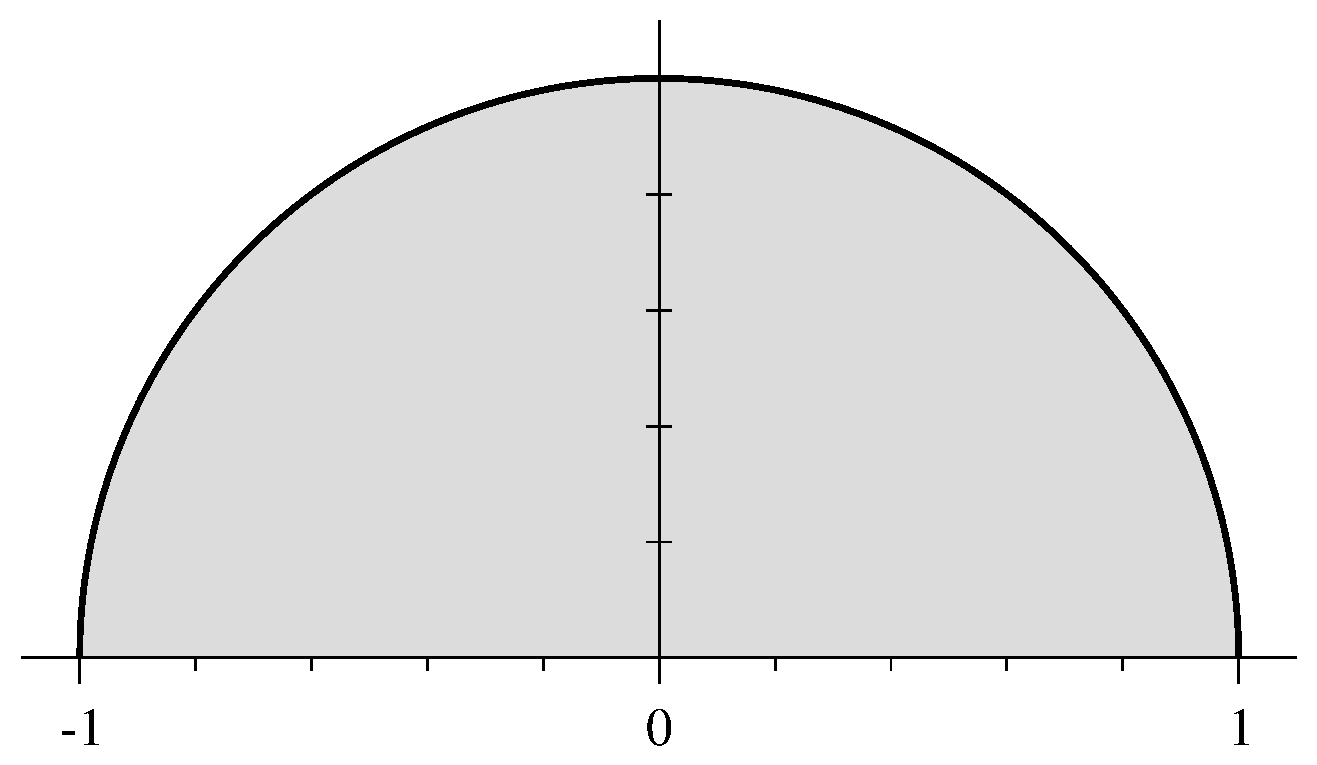
\includegraphics[width=9cm]{semicircle.eps}
\end{center}
\medskip and hence the value of the integral---the area under the
curve---must be $\half\pi=1.57079632679\ldots$

Alternatively, we can evaluate the integral on the computer by dividing the
domain of integration into a large number~$N$ of slices of width $h=2/N$
each and then using the Riemann definition of the integral:
\begin{displaymath}
I = \lim_{N\to\infty} \sum_{k=1}^N hy_k\,,
\end{displaymath}
where
\begin{displaymath}
y_k = \sqrt{1 - x_k^2}\qquad\mbox{and}\qquad
x_k = -1 + hk.
\end{displaymath}
We cannot in practice take the limit~$N\to\infty$, but we can make a
reasonable approximation by just making~$N$ large.
\begin{enumerate}
\item Write a program to evaluate the integral above with $N=100$ and
  compare the result with the exact value.  The two will not agree very
  well, because $N=100$ is not a sufficiently large number of slices.
\item Increase the value of~$N$ to get a more accurate value for the
  integral.  If we require that the program runs in about one second or
  less, how accurate a value can you get?
\end{enumerate}
Evaluating integrals is a common task in computational physics
calculations.  We will study techniques for doing integrals in detail in
the next chapter.  As we will see, there are substantially quicker and more
accurate methods than the simple one we have used here.

\end{exercises}

\end{document}
